% DOC OPTIONS
\documentclass[a4paper,12pt]{article} % Page Setup
\usepackage[portuguese]{babel} % Commands Language
\usepackage{graphicx} % Image Load
\usepackage{hyperref} % References
\usepackage[none]{hyphenat} % Remove Hyphenation
	\usepackage[left=2cm,right=2cm,bottom=5cm]{geometry} % Custom margin size

% Table of Contents Configuration
\setcounter{tocdepth}{3}

% DOCUMENT
\begin{document}

\begin{titlepage}
	\centering
	\Large \textbf{INSTITUTO POLITÉCNICO DE SETÚBAL} \\
	\normalsize \textbf{ESCOLA SUPERIOR DE TECNOLOGIAS DE SETÚBAL} \\
	\vspace{2cm}
	\begin{figure}[ht!]
		\centering
		
\includegraphics[scale=.5]{images/IPSLogo.png}
	\end{figure}
	\vspace{1cm}
	\Large \textbf{Qualidade de Software}\\
	\Large \textbf{Mestrado em Engenharia de Software}\\
	\vspace{1.5 cm}
	\Large Daniel Singh - 201901071\\
	\Large Rafael Marçalo - 201900456\\
	\vspace{.5cm}
	\large \today
\end{titlepage}

\newpage
\tableofcontents

\newpage
\listoffigures

\newpage
\listoftables

\newpage
\section{Introdução}
Este relatório tem como objetivo a análise da qualidade de código de um projeto realizado por outros alunos. Para esta análise iremos recorrer a uma breve experimentação das funcionalidades e requisitos do projeto.Em seguida iremos testar várias ferramentas e livrarias de análise da qualidade/consistência do código ao qual iremos em breve apresentar não só as suas funcionalidades, mas também os resultados que obtivemos com elas.

\newpage
\section{Análise do Caso de Estudo}
Sendo esta a primeira fase desta pequena investigação, transferimos o projeto caso de estudo do \footnote{Moodle IPS - \url{https://moodle.ips.pt/2324/}}{\textbf{Moodle}} e instalámos nas nossas máquinas para análise. Desta forma, após instalarmos e configurarmos o projeto nos nossos computadores, fizemos um breve teste das suas funcionalidades e diagnosticámos alguns problemas que possam afetar a qualidade do projeto, assim sendo, elaborámos uma lista de requisitos funcionais que o projeto deveria implementar.

\subsection{Análise de Requisitos}
\subsubsection{Clientes}
\begin{itemize}
	\item O sistema deverá permitir inserir novos clientes;
	\item O sistema deverá permitir pesquisar pelos clientes;
	\item O sistema deverá permitir aplicar filtros às pesquisas dos clientes;
	\item O sistema deverá permitir atualizar a informação dos clientes;
	\item O sistema deverá permitir eliminar clientes;
	\item O sistema deverá efetuar a validação de dados ao criar um cliente.
\end{itemize}

\subsubsection{Utilizadores}
\begin{itemize}
	\item O sistema deverá permitir inserir novos utilizadores;
	\item O sistema deverá permitir pesquisar pelos utilizadores;
	\item O sistema deverá permitir aplicar filtros às pesquisas dos utilizadores;
	\item O sistema deverá permitir atualizar a informação de outros utilizadores;
	\item O sistema deverá permitir eliminar outros utilizadores;
	\item O sistema deverá efetuar a validação de dados ao criar um utilizador.
\end{itemize}

\newpage
\subsubsection{Serviços}
\begin{itemize}
	\item O sistema deverá permitir criar serviços;
	\item O sistema deverá permitir pesquisar pelos serviços;
	\item O sistema deverá permitir realizar pesquisas filtrados aos serviços;
	\item O sistema deverá permitir aplicar filtros às pesquisas dos serviços;
	\item O sistema deverá permitir atualizar a informação dos serviços;
	\item O sistema deverá de validar os dados ao criar um serviço;
	\item O sistema deverá permitir reabrir um serviço concluído;
	\item O sistema deverá de mostrar quantos qual o index do serviço relativo à sua prioridade.
\end{itemize}

\subsubsection{Mensagens}
\begin{itemize}
	\item O sistema deverá permitir enviar mensagens para outros utilizadores em tempo real;
	\item O sistema deverá permitir escolher para qual utilizador.
\end{itemize}

\subsubsection{Sistema}
\begin{itemize}
	\item O sistema deverá permitir fazer login;
	\item O sistema deverá permitir fazer logout;
	\item O sistema deverá de verificar permissões no routing.
\end{itemize}

\newpage
\section{Ferramentas de Análise}
Após um diagnóstico de requisitos do projeto, avançamos para uma análise a nível de possíveis problemas de código, para esta tarefa, efetuamos uma pesquisa de ferramentas que nos possam ajudar com esta tarefa, das quais, achamos importante destacar:

\begin{itemize}
	\item \textbf{ESLint} é uma ferramenta de análise de código estático que verifica o código JavaScript procurando diversos problemas comuns, como erros de sintaxe, problemas de formatação, violações de estilo de código e possíveis bugs.

	\item \textbf{Prettier Code Formatter} é um formatador de código. Impõe um estilo consistente analisando seu código e reimprimindo-o conforme um conjunto de regras que levam em consideração diversos parâmetros como (comprimento máximo da linha, agrupando o código quando necessário, etc.). Utilizando esta ferramenta conseguimos garantir a uniformização do código desenvolvido ao longo do projeto.

	\item \textbf{Jest} é uma framework para testes de código compatível com bastantes projetos (Babel, TypeScript, Node, React, Angular, Vue e mais...). Suporta mocking, gera reports de code coverage.

	\item \textbf{Mocha} é outra framework de testes para Node capaz de correr no browser. Esta framework contém “interfaces” de testes que podem ser utilizados para vários tipos de desenvolvimento(TDD, BDD, exports, qunit, require, etc...). O Mocha também permite o fácil teste de funções assíncronas e de promises.

	\item \textbf{Chai}, livraria de testes especificada para testes do tipo BDD/TDD, esta livraria geralmente é integrada noutras frameworks específicas de testes(como o Mocha, por exemplo).
\end{itemize}

\newpage
\section{Linting}
Para a análise de linting do código usamos a ferramenta ESLint, devido à sua alta configurabilidade e por ser uma das ferramentas de linting mais utilizadas, como podemos observar no esquema abaixo:

\vspace{1cm}
\begin{figure}[ht!]
	\centering
	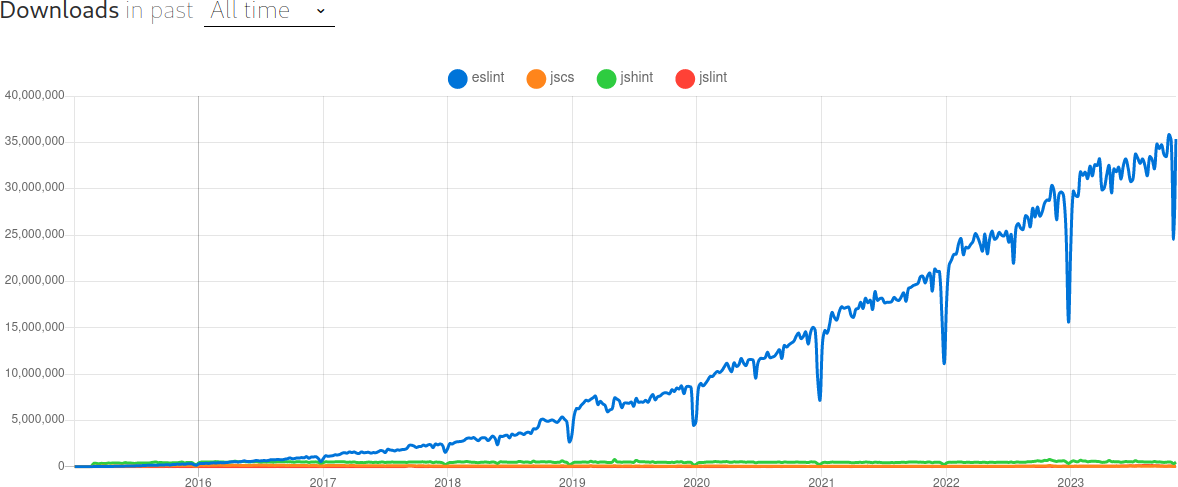
\includegraphics[scale=1.5]{images/lintTrend.png}
	\caption[Estatísticas de Download de Linters]{Estatísticas do download dos Linters ao longo do tempo\footnotemark}
\end{figure}
\footnotetext{Imagem obtida através de \url{https://npmtrends.com/eslint-vs-jscs-vs-jshint-vs-jslint}}

\newpage
\subsection{Resultados}
Através desta ferramenta, foi nos possível efetuar várias auditorias ao código utilizando várias configurações, permitindo-nos assim destacar as estatísticas

\subsubsection{Análise simples}
Para esta análise, configuramos o \textbf{ESLint} para apenas reportar erros de sintaxe e alguns problemas de código em geral(variáveis inutilizadas, valores \textit{undefined}, \textit{espaços} misturados com \textit{tabs}, etc...).

\vspace{1cm}
\begin{table}[!ht]
	\centering
	\begin{tabular}{|l|r|}
		\hline
		\textbf{Problema Anotado} & \textbf{Total} \\
		\hline
		Variáveis Inutilizadas & 40 \\
		\hline
		Valores \textit{undefined} & 189 \\
		\hline
		\textit{Espaços} Misturados com \textit{Tabs} & 2 \\
		\hline
	\end{tabular}
	\caption{Análise de Lint Simples}
\end{table}

\subsubsection{Análise simples (Client-side)}
Nesta análise decidimos fazer distinção entre problemas de código de cliente obtendo assim os seguintes resultados:

\vspace{1cm}
\begin{table}[!ht]
	\centering
	\begin{tabular}{|l|r|}
		\hline
		\textbf{Problema Anotado} & \textbf{Total} \\
		\hline
		Variáveis Inutilizadas & 23 \\
		\hline
		Valores \textit{undefined} & 189 \\
		\hline
		\textit{Espaços} Misturados com \textit{Tabs} & 2 \\
		\hline
	\end{tabular}
	\caption{Análise de Lint Simples (Client-side)}
\end{table}

\newpage
\subsubsection{Análise simples (Server-side)}
Nesta análise decidimos fazer distinção entre problemas de código de servidor obtendo assim os seguintes resultados:

\vspace{1cm}
\begin{table}[!ht]
	\centering
	\begin{tabular}{|l|r|}
		\hline
		\textbf{Problema Anotado} & \textbf{Total} \\
		\hline
		Variáveis Inutilizadas & 17 \\
		\hline
	\end{tabular}
	\caption{Análise de Lint Simples (Server-side)}
\end{table}

\subsubsection{Análise detalhada}
Para a análise detalhada, configuramos o \textbf{ESLint} para reportar os problemas da análise simples, assim como os problemas de estilo de código. Para esta análise, escolhemos os estilo de código \hyperlink{https://github.com/standard/standard}{\textit{Standard}} onde pudemos observar os seguintes resultados:

\vspace{1cm}
\begin{table}[!ht]
	\centering
	\begin{tabular}{|l|r|}
		\hline
		\textbf{Problema Anotado} & \textbf{Total} \\
		\hline
		Utilização de \textit{aspas} & 772 \\
		\hline
		Utilização de \textit{ponto e vírgula} & 1302 \\
		\hline
		\textit{Espaço} a terminar linha & 171 \\
		\hline
		Linhas em branco & 26 \\
		\hline
		Indentação incorreta & 2062 \\
		\hline
		\textit{Espaço} inserido várias vezes de seguida & 11 \\
		\hline
		\textit{Espaço} inserido antes de comentário & 50 \\
		\hline
		\textit{Espaço} em falta antes do \textit{parênteses} da \textit{função} & 121 \\
		\hline
		\textit{Espaço} em falta antes de blocos de código & 67 \\
		\hline
		Operador ternário desnecessário & 1 \\
		\hline
		Trocar variável para \textit{const} & 1 \\
		\hline
		Usar \textit{var} & 11 \\
		\hline
		\textit{Espaço} antes de uma palavra-chave & 2 \\
		\hline
		Estilo das \textit{chavetas} & 93 \\
		\hline
		\textit{Espaço} entre as \textit{=>} & 85 \\
		\hline
		\textit{Objeto} abreviado & 6 \\
		\hline
		Caractere terminal de ficheiro & 5 \\
		\hline
		\textit{Espaço} dentro da definição de objeto & 5 \\
		\hline
		Variáveis Inutilizadas & 11 \\
		\hline
		\textit{Espaços} \textit{padding} blocos de código & 7 \\
		\hline
		\textit{Hardcoded callback} & 24 \\
		\hline
		Valores \textit{undefined} & 189 \\
		\hline
		Propriedades sem \textit{aspas} & 6 \\
		\hline
		\textit{Tabs} vazios & 2 \\
		\hline
		Nova linha após \textit{parênteses} de objeto & 9 \\
		\hline
		Nova linha após propriedade de objeto & 9 \\
		\hline
		Falta de \textit{espaços} entre operadores lógicos e aritméticos & 22 \\
		\hline
		\textit{Vírgula} em propriedades finais de objetos & 2 \\
		\hline
		\textit{Espaços} entre parênteses & 2 \\
		\hline
		\textit{Espaços} múltiplos & 2 \\
		\hline
	\end{tabular}
	\caption{Análise de Lint Detalhada}
\end{table}
\end{document}
